\documentclass[ %
10pt, % Schriftgroesse
a4paper, % Papiergroesse
headsepline, % Kopfzeilenlinie
footsepline, % Fusszeilenlinie
%parskip, % Abstand zw. Absaetzen
headings=normal, % etw. kleinere Ueberschriften
parskip=full,
%draft % Testkram
]{scrreprt}
% packages
\usepackage[utf8x]{inputenc}
\usepackage[T1]{fontenc}
\usepackage{ucs}
\usepackage[ngerman]{babel}
\usepackage{url} % Schönere URLs
\usepackage{graphicx} % Grafiken
%\usepackage{microtype} % Schoenere Blocksatzraender
\usepackage[ngerman]{varioref} % Tolle Verweise
\usepackage[german]{fancyref} % Tolle Verweise V2
\usepackage{hyperref}
%\usepackage{fancyhdr} % Kopf- und Fusszeilen
\usepackage[automark]{scrpage2} % Kopf- und Fusszeilen
\usepackage[top=2cm, bottom=4cm, lmargin=2cm,rmargin=2cm, footskip=1.5cm]{geometry} % Seitenraender
\usepackage[locale=DE,alsoload=binary]{siunitx} % Einheiten
% Entwurf
\usepackage{color} % Paket für verschiedene Farben
\usepackage{eso-pic}
\usepackage{wallpaper}
\usepackage{tikz}
\usepackage{rotating}
\usepackage{blindtext}

\newcommand{\makedate}{15. April 2013}

\usetikzlibrary{matrix,fadings,calc,positioning,
				decorations.pathreplacing,arrows,shapes}

\definecolor{lightgray}{gray}{.75}

\definecolor{dlrgblue}{cmyk}{.98,.47,0,.3}

\author{}%Einsatz}
%\title{Dienstanweisung}
\title{}
\date{}%Stand: \makedate}
\publishers{}%Landesverband Niedersachsen\\Bezirk Cuxhaven-Osterholz\\Ortsgruppe Langen e.V.}
%\publishers{Ortsgruppe Langen e.V.}


%{
%\AddToShipoutPicture{%
%\AtTextCenter{%
%\makebox(0,0)[c]{\resizebox{\textwidth}{!}{%
%\rotatebox{45}{\textsf{\textbf{\color{lightgray}Entwurf}}}}}
%}
%}
%}

\newcommand{\changefont}[3]{
\fontfamily{#1} \fontseries{#2} \fontshape{#3} \selectfont}

\newcommand{\erganzung}{}
\newcommand{\dienstanweisung}{Übersicht}




\pagestyle{scrheadings}
% \ihead{Technik/Einsatz}
% \ohead{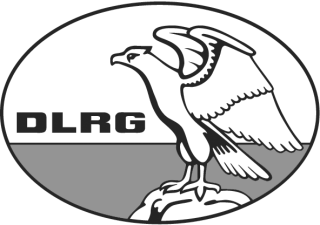
\includegraphics[height=\headheight]{Logo-B-Graustufen}}
\ihead{DLRG OG Langen e.V.}
\ohead{Technik/Einsatz}
\ifoot{\dienstanweisung \erganzung}
\cfoot{Stand: \makedate}
\ofoot{\pagemark}

\begin{document}
\changefont{cmss}{m}{n}
%\maketitle
%\tableofcontents
%\addtocontents{toc}{\protect\thispagestyle{scrheadings}} 
% \addpart{Allgemeines zur Dienstanweisung}
% \thispagestyle{empty}
%\include{Allgemeines}
%\include{WRD}
%\include{WRD-Mat}
%\end{document}
\renewcommand{\dienstanweisung}{DA\,4-01/2013}
\addchap{Wasserrettungsdienst}
\thispagestyle{scrheadings}
\addsec{Allgemeines}
Ein normaler Wachdienst besteht aus vier Personen: ein Wachführer und drei Wachgänger. Die Mindestbesatzung der Wasserrettungsstation am Sieverner See besteht aus zwei Personen. Maximal sollten sechs Personen anwesend sein. Ausnahmen kann die Leitung Einsatz oder der Wachführer nach Rücksprache mit der Leitung Einsatz festlegen.

Jeder auf der Wasserrettungsstation eingesetzte Wasserretter sollte bedenken, dass er die DLRG nach außen repräsentiert und sein Verhalten das Ansehen der DLRG bestimmt.

Jede im WRD eingesetzte Person hat ihre ABC-Ausrüstung bereitzuhalten.

Im WRD eingesetzte Kräfte sind den Badegästen gegenüber nicht weisungsbefugt, jedoch verpflichtet, sie auf Gefahren hinzuweisen.  Ausnahmen regeln die örtlichen Gesetze und Verordnungen.

Jeglicher Genuss von Alkohol oder anderen berauschenden Mitteln unmittelbar vor und während der Ausübung des WRD ist für alle im Dienst befindlichen Personen ausdrücklich untersagt. Dies gilt auch für dritte Personen, die sich auf der Wasserrettungsstation aufhalten.

\addsec{Personal und Diensteinteilung}
Der Wachführer wird vom Leiter Einsatz der Gliederung bestimmt. Der Wachführer ist ein geeigneter Wasserretter mit dem erfolgreich abgeschlossenen Ausbildungsgang \glqq Wachführer\grqq\, gemäß gültiger Prüfungsordnung (PO) WRD, dort 4.3.1. Alte Ausbildungsgänge (Wachleiter gemäß PO WRD, dort 4.3.1 oder 4.8.1) behalten ihre Gültigkeit. Alternativ ist der Wachführer ein geeigneter Wasserretter mit dem erfolgreich abgeschlossenen Ausbildungsgang \glqq Fachausbildung Wasserrettungsdienst\grqq\, gemäß gültiger PO WRD, dort 4.1.1, der das 18. Lebensjahr vollendet hat. Der Wachführer sollte außerdem einen gültigen Sanitätslehrgang A (gemäß gültiger PO EH/SAN, dort 3.3.1) oder höhere Qualifikation besitzen. Wasserretter ohne Ausbildung können aufgrund ihrer langjährigen Erfahrung im WRD als Wachführer eingesetzt werden. Ist der Wachführer kein ausgebildeter Wachführer, hat er mindestens einmal in zwei Jahren an einer Wachführereinweisung teilzunehmen.

Die zugehörigen Wachgänger werden ebenfalls vom Leiter Einsatz der Gliederung bestimmt. Wachgänger sind geeignete Rettungsschwimmer mit einem \glqq Deutschen Rettungsschwimmabzeichen – Bronze\grqq\, (gemäß gültiger PO S/RS, dort 1.5.1), nicht älter als zwei Jahre, und Erste-Hilfe-Lehrgang (gemäß gültiger PO EH/SAN, dort 3.1.2), nicht älter als zwei Jahre, oder höherer Ausbildung.

Die Bestimmung des Wachführers und der Wachgänger kann vom Leiter Einsatz an einen geeigneten Beauftragten delegiert werden. Die Bestimmung der Wachgänger kann auch durch den jeweiligen Wachführer durchgeführt werden.

Jede im Wasserrettungsdienst der OG Langen eingesetzte Kraft sollte an einer Wacheinweisung teilgenommen haben, um die Besonderheiten der Wasserrettungsstation und des Wachgebietes kennenzulernen. 
Eine regelmäßige Auffrischung dieser Wacheinweisung sollte vorgenommen werden. 
Empfohlen ist eine jährliche Wiederholung, sie sollte mindestens alle zwei Jahre oder wenn es relevante Neuerungen im Bereich des WRD gibt stattfinden. 
Die Wacheinweisung sollte von einem Ausbilder oder Multiplikator WRD (gemäß gültiger PO WRD, dort 4.8.1 oder 4.9.1) durchgeführt werden. 
Genaueres wird von der Leitung Einsatz der Gliederung festgelegt.

Bei der Diensteinteilung sind die Wünsche des Personals gleichgestellt zu berücksichtigen. Höher qualifizierte Kräfte sind vorzuziehen.

Die Diensteinteilung ist im Online-Wachdienstplan der OG Langen vorzunehmen. Dessen Adresse\footnote{\url{https://wachplan.dlrg-langen.de}} wird von der Leitung Einsatz der OG Langen bekannt gegeben.

\addsec{Bekleidung}
Es ist dem Wetter angemessene Einsatzkleidung gemäß DLRG-Standards zu tragen. Genauere Informationen dazu finden sich in Anhang \vref{appendix:kleidung}.
ie gewählte Einsatzkleidung darf den Wachgänger in keinster Weise bei der Ausübung seiner Tätigkeiten einschränken. Insbesondere ist bei Badebetrieb darauf zu achten, dass ein schwimmerischer Einsatz jederzeit möglich ist.

\addsec{Wachführer}
Der Wachführer ist für die ordnungsgemäße Durchführung des WRD verantwortlich und im Rahmen dieser Aufgabe gegenüber den eingesetzten Kräften weisungsbefugt. Seinen Anordnungen ist Folge zu leisten. Er hat u.a. die Diensteinteilung vor Ort vorzunehmen. Die Wünsche des Personals sollten dabei berücksichtigt werden.

Der Wachführer ist für die Einhaltung aller Gesetze, Ordnungen, Satzungen, DLRG-Anweisungen und Bestimmungen durch die eingesetzten Kräfte verantwortlich.
 
\addsec{Wachdienstzeiten}
Die Wachsaison beginnt alljährlich am 15.\,Mai und endet am 15.\,September. Innerhalb dieser Zeit findet der Wachdienst statt. Zu Beginn dieser Zeit sollte die Wacheinweisung durchgeführt werden. Außerhalb dieser Zeit findet der Wachdienst nur in Ausnahmefällen statt.

Für die OG Langen werden folgende grundsätzliche Wachdienstzeiten festgelegt:

\subsection*{Außerhalb niedersächsischer Schulferien}
\begin{tabular}{lr}
Freitag  & 14:00 -- 18:00 Uhr\\
Samstag, Sonn- u. Feiertag & 10:00 -- 18:00 Uhr
\end{tabular}
\subsection*{Innerhalb niedersächsischer Schulferien}
\begin{tabular}{lr}
Montag--Freitag & 10:00 -- 18:00 Uhr\\
Samstag, Sonn- u. Feiertag & 10:00 -- 18:00 Uhr
\end{tabular}
\subsection*{Schichten}
Diese Zeiten sind in zwei Schichten aufgeteilt:\\
\begin{tabular}{lr}
Frühschicht   & 10:00 -- 14:00 Uhr\\
Spätschicht   & 14:00 -- 18:00 Uhr
\end{tabular}

Grundsätzlich hat der WRD bei gutem Wetter stattzufinden. Der Wachführer entscheidet ggf. in Rücksprache mit der Leitung Einsatz der Gliederung, ob der WRD stattfindet. Neben dem Wetter sollte auch die Besucherzahl im Wachgebiet zur Entscheidungsfindung herangezogen werden. Die Spätschicht ist innterhalb der Schulferien täglich ab 20 °C, außerhalb der Schulferien nur an Freitagen, Wochenenden und Feiertagen unter gleichen Bedingungen zu besetzen.

Falls erforderlich, muss die Wachdienstzeit entsprechend erweitert werden. Die Verlängerung des WRD obliegt der Leitung Einsatz der Gliederung oder dem jeweiligen Wachführer.

Auf Anweisung des Wachführers haben die Wachgänger bis zu 30 Minuten vor Dienstbeginn zu erscheinen. In diesem Zeitraum hat der Wachführer die Möglichkeit, Übungen und Training durchzuführen, die die Einsatzfähigkeit der Wachgänger erhalten oder verbessern.


\addsec{Wachbuch}
Das Wachbuch ist sorgfältig zu führen und vom Wachführer gegenzuzeichnen. An- und Abwesenheitszeiten aller eingesetzten Kräfte sind halbstündlich im Wachbuch festzuhalten.

\addsec{Flagge}
Während des WRD sind die DLRG-Flagge und die rot-über-gelbe Flagge zu hissen. Im Falle eines Gewitters o.ä. Gefährdung für die Badegäste ist die rot-über-gelbe Beflaggung möglichst (unter Beachtung der UVV und des Eigenschutzes) unverzüglich einzuholen.

\addsec{Einsätze}
Im Falle eines Einsatzes ist dieser in das Verbandbuch einzutragen. 
Ggf. ist ein Erste-Hilfe-Protokoll anzulegen. 
Lebensrettungen oder schwere Unfälle sind unverzüglich der Leitung Einsatz der Gliederung zu melden. 
Bei Erste-Hilfe-Leistungen ist dem Patienten grundsätzlich ein Arztbesuch bzw. das Aufsuchen eines Krankenhauses zu empfehlen. 
Sollte dieser dieses verweigern, so ist das entsprechende Formblatt auszufüllen und zur rechtlichen Absicherung durch den Patienten zu unterzeichnen. 
Dies kann bei geringfügigen Erste-Hilfe-Leistungen unterlassen werden.

Wasserrettungseinsätze und andere größere Einsätze sind nach dem im Anhang \vref{appendix:ablaufplan} angefügten Ablaufplan durchzuführen.

\addsec{Wasserrettungsstation}
Das Material der Wasserrettungsstation ist jederzeit einsatzbereit zu halten. Der Wachführer ist für die Funktionsfähigkeit und Vollständigkeit des Materials verantwortlich. Das zur Verfügung gestellte Material ist schonend zu behandeln. Mängel sind umgehend der Leitung Einsatz der Gliederung zu melden.  Bei Abhandenkommen durch Diebstahl ist bei der zuständigen Polizeidienststelle umgehend eine Strafanzeige zu erstatten. 

Verderbliche Lebensmittel sind nicht auf Dauer in der Wasserrettungsstation zu lagern. Die Wasserrettungsstation ist sauber zu verlassen. Am Wochenende, vor längeren Schlechtwetterperioden und bei Saisonschluss ist die Wasserrettungsstation gründlich zu reinigen.

\addsec{Übernachtungen in der Wasserrettungsstation}
Übernachtungen in der Wasserrettungsstation sind grundsätzlich nicht gestattet. Über Ausnahmen von dieser Regelung entscheidet die Leitung Einsatz nach Anfrage mindestens zwei Tage vor dem Tag der Übernachtung. 

\addsec{Auftreten und Verhalten}
Während des Wachdienstes ist das Tor zum Seegelände abzuschließen, um unbefugtes Befahren des Geländes zu verhindern. Das Tor muss nach dem Wachdienst (und im Einsatzfall) wieder geöffnet werden, um den Rettungsweg nicht zu behindern.

Der Hintereingang der Wasserrettungsstation ist während des Wachdienstes abzuschließen, die vordere Tür und die Jalousien sind zu öffnen.

Das Rettungsbrett ist während der Dienstzeit nah am Seeufer auf dem Laufweg zum Wasser zu platzieren, um eine kurze Einsatzzeiten zu gewährleisten. Sind viele Besucher zu erwarten, ist auch das Boot an das Seeufer zu bringen, um den Badebetrieb ggf. von der Wasserseite überwachen zu können.

Vor dem Beginn des Wachdienstes sind Funkgeräte, Material und Sanitätstasche auf Einsatzfähigkeit und Vollständigkeit zu überprüfen.

Die Aufmerksamkeit ist auf das Geschehen auf bzw. am See zu richten. Regelmäßige Kontrollgänge sind zu zweit über das Seegelände durchzuführen. 

Der Wachdienstbereich der Wasserrettungsstation ist grundsätzlich nur alleine zu verlassen, bspw. für Toilettengänge oder Essenszubereitung. Nicht dem Wachdienst zugeordnete Tätigkeiten sollten nicht im öffentlich einsehbaren Bereich der Wasserrettungsstation durchgeführt werden. Dies ist jedoch nur gestattet, wenn die Bewachung des Wachgebiets ausreichend gewährleistet ist. 

\addsec{Unfälle}
Die für die DLRG geltenden Unfallverhütungsvorschriften sind zu beachten. Hat ein Wachgänger einen Körper-- oder Sachschaden in Ausübung des WRD erlitten, so ist dieses binnen zwei Tagen der Leitung Einsatz der Gliederung zu melden. Der entsprechende Unfallmeldebogen ist auszufüllen.

Entstehen während der Ausübung des WRD Schadensersatz-- bzw. Haftungsansprüche von Seiten Dritter, so sind diese ohne Schuldeingeständnisse oder sonstige Zugeständnisse (mündlich oder schriftlich) gegenüber Dritten dem Vorstand der Gliederung zu melden. Als Auskunftspersonen sind der Vorstand bzw. der Justiziar zu benennen. Soweit Geschehnisse festgehalten werden, sind diese dem Schadengegner ohne vorherige Rücksprache mit den genannten Stellen grundsätzlich nicht gegenzuzeichnen oder auszuhändigen.

\addsec{Sprechfunk}
Im Bereich der DLRG Ortsgruppe Langen e.V. sind ausschließlich die durch den DLRG Bezirk Cuxhaven--Osterholz e.V. vergebenen OPTA zu verwenden. Diese beginnt mit der Organisationskennung der DLRG Ortsgruppe Langen e.V. (72). Beispiel für eine OPTA: \glqq Adler Langen 72--00--3\grqq{} (Hauptwache)

In einer Übergangsphase bis zum 31.12.2013 sind noch die bisher geführten Rufnahmen gestattet, jedoch sind OPTA--Kennungen zu bevorzugen.

\addsec{Material im Wasserrettungsdienst}
\subsection*{Allgemeines}
Um die bestmögliche Versorgung von Verletzten, Verunfallten sowie der Wachgänger zu gewährleisten, sollte die Wasserrettungsstation mit dem im Folgendem aufgeführten Material ausgestattet sein. 

\subsection*{Sanitätsmaterial}
Die Wasserrettungsstation ist mit einer Sanitätstasche auszustatten. Deren Inhalt ist dem Abschnitt Material im Bereich 3-01 (Sanitätsdienst) dieser DA zu entnehmen. 

Der Sanitätsschrank sollte mit weiteren Sanitätsmaterialien ausgestattet sein.

Die Station selbst sollte mit einer möglichst höhenverstellbaren Liege mit verstellbarer Kopfstütze ausgestattet sein. 
Es ist außerdem eine Trage zum Patiententransport vorzuhalten.

\subsection*{Wasserrettungsmaterial}
Um den Wasserrettungsdienst durchführen zu können, sind folgende Materialien vorzuhalten:\begin{itemize}
\item ein Rettungsboot
\item ein Rettungsbrett zum schnellen Anschwimmen von Verunfallten
\item ein Spineboard zum sicheren Transport von Wirbelsäulenpatienten
\item ein Gurtretter
\item eine Rettungsboje
\end{itemize}

\subsection*{Wachgängerversorgung und -sicherheit}
Zur Versorgung der Wachgänger hat die Wasserrettungsstation eine Küche. Diese Küche enthält einen Herd mit diversen Töpfen, eine Mikrowelle, einen Kühlschrank und eine Spüle. 
Geschirr ist vorzuhalten.

Um Verletzungen durch Sonneneinstrahlung vorzubeugen, ist die Dachplattform mit einem Sonnenschutz auszustatten. Weiterhin ist in der Wasserrettungsstation Sonnencreme vorzuhalten.

\subsection*{Sonstiges}
Das Einsatzmaterial ist einsatzklar zu lagern. Fehlende und defekte Materialien sind der Leitung Einsatz zu melden. 

\vspace*{\fill}
\begin{tabular}{lcr}
Langen, der \makedate & & \dotfill \\
 & \hspace{4cm} & \hspace{4cm} Unterschrift des Vorsitzenden
\end{tabular}

\appendix
\chapter{Einsatzablauf}\label{appendix:ablaufplan}
\renewcommand{\erganzung}{ (Anhang)}
\thispagestyle{scrheadings}
\addsec{Wasserrettungseinsatz}
\begin{tikzpicture}
	[mybox/.style={
		rectangle,rounded corners=1mm,minimum size=6mm,anchor=base,
		very thick,draw=black!50,top color=white,bottom color=black!20},
	ybox/.style={
		rectangle,rounded corners=1mm,minimum size=6mm,anchor=base,
		very thick,draw=black!50,top color=white,bottom color=yellow!20},
	bbox/.style={
		rectangle,rounded corners=1mm,minimum size=6mm,anchor=base,
		very thick,draw=black!50,top color=white,bottom color=blue!20},
	rbox/.style={
		rectangle,rounded corners=1mm,minimum size=6mm,anchor=base,
		very thick,draw=black!50,top color=white,bottom color=red!20},
	gbox/.style={
		rectangle,rounded corners=1mm,minimum size=6mm,anchor=base,
		very thick,draw=black!50,top color=white,bottom color=green!20},
	wbox/.style={
		rectangle,rounded corners=1mm,minimum size=6mm,anchor=base,
		very thick,draw=black!50,top color=white,bottom color=white!20},
	nobox/.style={
		rectangle,rounded corners=1mm,minimum size=6mm,anchor=base,
		very thick,draw=white!50,top color=white,bottom color=white!20},
	circle/.style={
		draw,ellipse}]

	\node (wr1) [rbox] {Wasserretter 1};
	\node (wr2) [rbox, right=2cm of wr1] {Wasserretter 2};
	\node (wr3) [wbox, right=2cm of wr2] {Wasserretter 3};
	\node (wf) 	[bbox, right=2cm of wr3] {Wachführer};
	
	\node (aus) [ybox, below=of wr1] {\parbox{2.5cm}{Ausrüstung (Rettungsbrett) aufnehmen}};
	\node (mel) [bbox, below=of wr2] {\parbox{2.5cm}{Meldung an den Wachführer\\ }};
	\node (san) [gbox, below=of wr3] {\parbox{2.5cm}{San-Ausrüstung ans Ufer\\ }};
	
	\node (h20) [ybox, below=5mm of aus] {\parbox{2.5cm}{ins Wasser \& anschwimmen\\ }};
	\node (ruk) [bbox, below=5mm of mel] {\parbox{2.5cm}{Rückmeldung WF abwarten\\ }};
	\node (unt) [gbox, below=5mm of san] {\parbox{2.5cm}{zur Unterstützung zum Anlandebereich}};
	
	\node (sic) [ybox, below=5mm of h20] {\parbox{2.5cm}{Sichern an der Wasseroberfläche}};
	\node (abc) [bbox, below=5mm of ruk] {\parbox{2.5cm}{ABC--Ausrüstung aufnehmen}};
	
	\node (h21) [bbox, below=5mm of abc] {\parbox{2.5cm}{ins Wasser \& anschwimmen}};
	
	\node (rt2) [ybox, below=19.4mm of sic] {\parbox{2.5cm}{Rücktransport d. Verunfallten z. Ufer}};
	\node (rtr) [bbox, below=5mm of h21] {\parbox{2.5cm}{Rücktransport d. Verunfallten z. Ufer}};
	
	\node (ve1) [ybox, below=5mm of rt2] {\parbox{2.5cm}{Versorgung des Patienten an Land}};
	\node (ve2) [bbox, below=5mm of rtr] {\parbox{2.5cm}{Versorgung des Patienten an Land}};
	\node (ve3) [gbox, below=57.2mm of unt] {\parbox{2.5cm}{Versorgung des Patienten an Land}};
	
	\node (ubg) [gbox, below=5mm of ve3] {\parbox{2.5cm}{Übergabe an den Landrettungsdienst}};
	
	% Wachfuehrergedoens	
	\node (ela) [wbox, below=of wf]  {\parbox{2.5cm}{eigene Lage}};
	\node (gef) [wbox, below=1mm of ela] {\parbox{2.5cm}{Gefahrenlage}};	
	\node (tak) [wbox, below=1mm of gef] {\parbox{2.5cm}{taktische Entscheidung}};
	\node (kra) [wbox, below=1mm of tak] {\parbox{2.5cm}{Kräfte ausreichend?}};
	\node (not) [wbox, below=1mm of kra] {\parbox{2.5cm}{Notruf}};
	\node (vog) [wbox, below=95mm of not] {\parbox{2.5cm}{Leitung Einsatz informieren}};
	\node (pre) [wbox, below=5mm of vog] {\parbox{2.5cm}{Umgang mit der Presse}};
	
	% Unfallereignis
	\node (beo) [circle, below right=2mm and -1mm of wr1] {Unfallereignis};
	
	% Erstgespreaech
	\node (egs) [wbox, below right=5mm and -11.7cm of ubg] {\parbox{15.6cm}{\centering Erstgespräch/Einsatznachbesprechung}};
	
	% Einsatzdoku
	\node (doku) [wbox, left=1mm of tak] {\begin{sideways}\parbox{2.5cm}{Einsatz-dokumentation}\end{sideways}};
\end{tikzpicture}

\chapter{Einsatzkleidung}\label{appendix:kleidung}
\thispagestyle{scrheadings}
\addsec{Sommerkleidung}
Die Sommerbekleidung besteht aus einem roten oder gelben DLRG--Shirt mit dem Rückenaufdruck \glqq Wasserrettung\grqq{} und einer roten Shorts mit dem DLRG--Wortmarkenaufdruck.
Darunter ist eine Badehose oder ein Badeanzug zu tragen.
\addsec{Lange Bekleidung}
Die lange Bekleidung besteht aus einem \glqq Anorak Wasserrettung Standard I\grqq{} der DLRG--Materialstelle und einer \glqq Einsatzhose Herren/Damen mit Reflex\grqq{} der DLRG--Materialstelle. Als Schuhe werden Sicherheitsschuhe nach dem Standard S3 empfohlen.
\addsec{Qualifikationsabzeichen}
Qualifikationsabzeichen und Rückenschilder dürfen nur von Personen getragen werden, die die Gültigkeit der jeweiligen Qualifkation nachweisen können. Ein Qualifikationsabzeichen sollte möglichst die ausgeübte Qualifikation, kann jedoch auch die höchste gültige Qualifikation darstellen. Im Wasserrettungsdienst ist grundsätzlich das Rückenschild \glqq Wasserrettung\grqq{} zu tragen. Dies gilt nicht für Einsatzwesten. Dort findet die gleiche Regel wie bei Qualifikationsabzeichen Anwendung.
\addsec{Zusätzliche Bekleidung}
Weiterhin können getragen werden: \begin{itemize}
\item DLRG--Pullover in rot mit Rückenaufdruck \glqq Wasserrettung\grqq{}
\item DLRG--Wetterbekleidung leicht/schwer
\item weitere PSA
\end{itemize}

\end{document}